%%%%%%%%%%%%%%%%%%%%%%%%%%%%%%%%%%%%%%%%%%%%%%%%%%%%%%%%%%%%%%%%%%%%%%%%%%%

\documentclass{standalone}

\usepackage{mathptmx}
\usepackage{tikz}
\usetikzlibrary{decorations.pathreplacing}
\usetikzlibrary{external}
\tikzexternalize{model}

%% We default to Times.
\renewcommand{\rmdefault}{ptm}
\renewcommand{\ttdefault}{pcr}
%% enable Times/Palatino main text font
\normalfont\selectfont

\begin{document}
%%
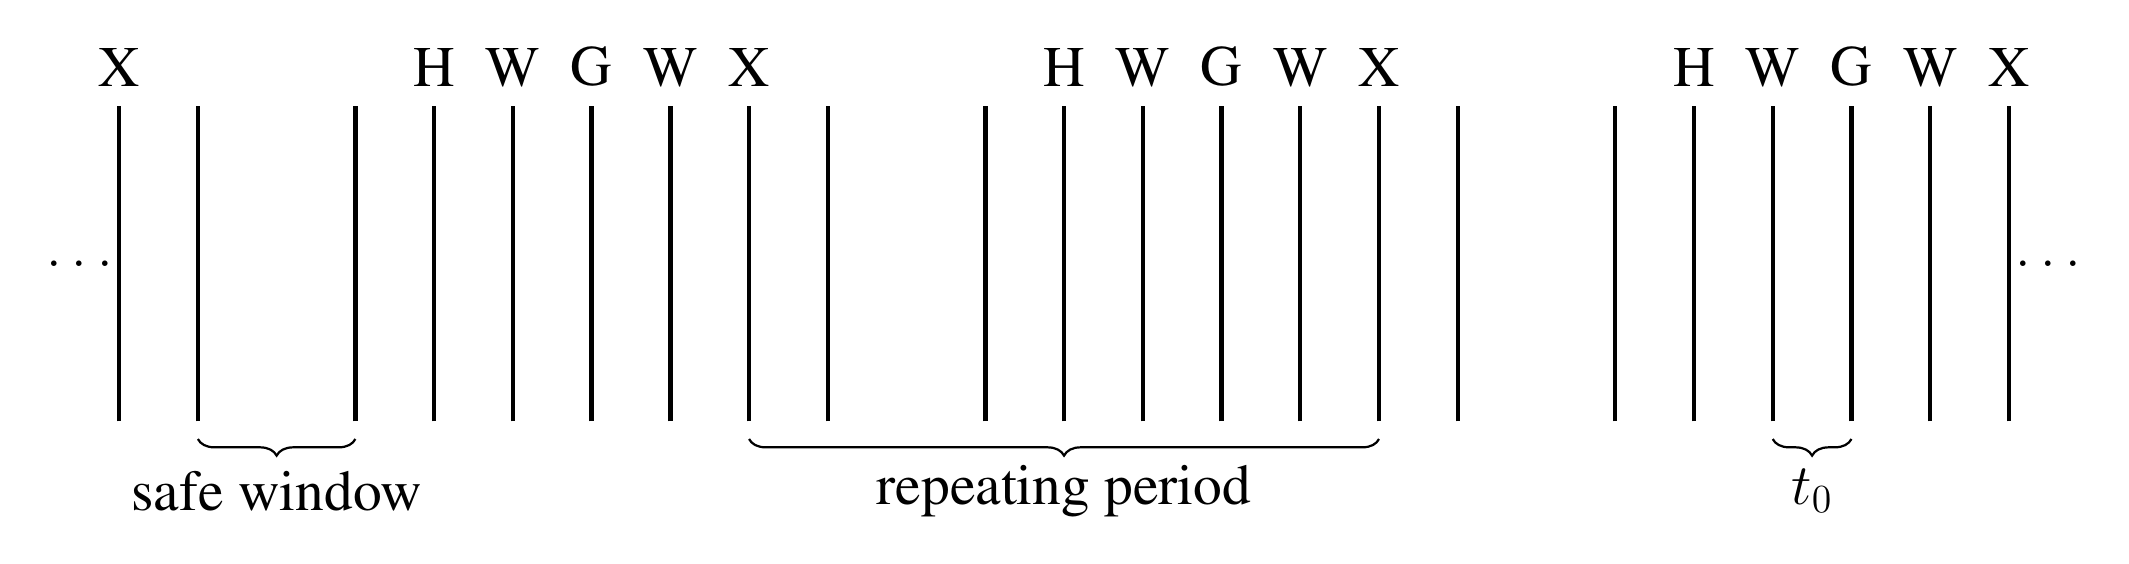
\begin{tikzpicture}[%%
  arrowDecorate/.style={-,thick},%%
  braceDecorate/.style={%%
    decorate,thick,decoration={brace,amplitude=6pt,mirror,raise=4pt}%%
  },%%
  lineDecorate/.style={-,ultra thick},%%
  nodeDecorate/.style={black,midway,yshift=-0.8cm,align=center}%%
]
\huge
%% 
%% Global variables.
\pgfmathsetmacro{\dx}{1}
\pgfmathsetmacro{\dy}{0.25}
\pgfmathsetmacro{\X}{0}
\pgfmathsetmacro{\Ya}{0}
\pgfmathsetmacro{\Yb}{4}
%%
%% Left ellipsis.
\node[] () at (\X-\dx/2,\Yb/2) {$\dots$};
%%
%% Left-most window.
\draw[lineDecorate] (\X,\Ya) edge (\X,\Yb);
\draw[lineDecorate] (\dx,\Ya) edge (\dx,\Yb);
\node[above] at (\X,\Yb) {X};
%%
%% Label the left safe window.
\pgfmathsetmacro{\safeLXa}{\dx}
\pgfmathsetmacro{\safeLXb}{3*\dx}
\pgfmathsetmacro{\safeLYa}{\Ya-\dy/3}
\pgfmathsetmacro{\safeLYb}{\safeLYa}
\draw[braceDecorate] (\safeLXa,\safeLYa) -- (\safeLXb,\safeLYb)
  node [nodeDecorate] {safe window};
%%
%% Left window.
\draw[lineDecorate] (\safeLXb,\Ya) edge (\safeLXb,\Yb);
\foreach \x/\ell in {1/H,2/W,3/G,4/W,5/X} {
  \draw[lineDecorate] (\safeLXb+\x,\Ya) edge (\safeLXb+\x,\Yb);
  \node[above] at (\safeLXb+\x,\Yb) {\ell};
}
\draw[lineDecorate] (\safeLXb+6,\Ya) edge (\safeLXb+6,\Yb);
%%
%% Middle safe window.
\pgfmathsetmacro{\safeMXa}{\safeLXb+6}
\pgfmathsetmacro{\safeMXb}{\safeMXa+2}
%%
%% Middle window.
\draw[lineDecorate] (\safeMXb,\Ya) edge (\safeMXb,\Yb);
\foreach \x/\ell in {1/H,2/W,3/G,4/W,5/X} {
  \draw[lineDecorate] (\safeMXb+\x,\Ya) edge (\safeMXb+\x,\Yb);
  \node[above] at (\safeMXb+\x,\Yb) {\ell};
}
\draw[lineDecorate] (\safeMXb+6,\Ya) edge (\safeMXb+6,\Yb);
%%
%% Label a repeating period.
\pgfmathsetmacro{\periodXa}{\safeLXb+5}
\pgfmathsetmacro{\periodXb}{\safeMXb+5}
\pgfmathsetmacro{\periodYa}{\safeLYa}
\pgfmathsetmacro{\periodYb}{\safeLYb}
\draw[braceDecorate] (\periodXa,\periodYa) -- (\periodXb,\periodYb)
  node [nodeDecorate] {repeating period};
%%
%% Right safe window.
\pgfmathsetmacro{\safeRXa}{\safeMXb+6}
\pgfmathsetmacro{\safeRXb}{\safeRXa+2}
%%
%% Right window.
\draw[lineDecorate] (\safeRXb,\Ya) edge (\safeRXb,\Yb);
\foreach \x/\ell in {1/H,2/W,3/G,4/W,5/X} {
  \draw[lineDecorate] (\safeRXb+\x,\Ya) edge (\safeRXb+\x,\Yb);
  \node[above] at (\safeRXb+\x,\Yb) {\ell};
}
% \draw[lineDecorate] (\safeRXb+6,\Ya) edge (\safeRXb+6,\Yb);
%%
%% Label a time buffer.
\pgfmathsetmacro{\bufferXa}{\safeRXb+2}
\pgfmathsetmacro{\bufferXb}{\safeRXb+3}
\pgfmathsetmacro{\bufferYa}{\periodYa}
\pgfmathsetmacro{\bufferYb}{\periodYb}
\draw[braceDecorate] (\bufferXa,\bufferYa) -- (\bufferXb,\bufferYb)
  node [nodeDecorate] {$t_0$};
%%
%% Right ellipsis.
\node[] () at (\safeRXb+6-\dx/2,\Yb/2) {$\dots$};
\end{tikzpicture}

\end{document}
